% !TeX spellcheck = fr_FR
\begin{resume}
La gestion de l'hétérogénéité peut (et doit) être considérée sous plusieurs aspects. Alors que le chapitre précédent a donné des exemples de travaux dans lesquels l'étude sur l'hétérogénéité s'était concentrée sur les aspects liés à la communication, dans ce chapitre nous nous concentrons sur l'hétérogénéité de calcul. Ce type d'hétérogénéité est souvent le plus simple à traiter car le plus fréquent : il est presque impossible de développer une application parallèle dans laquelle les tâches de calcul sont parfaitement régulières. Bien, sûr, la gestion des tâches régulières ou irrégulières dépend de leur interdépendance. Plus elles sont découplées, moins on trouve de contraintes pour leur exécution, ce que simplifie leur gestion.

Dans ce chapitre nous considérons que les tâches de calcul sont hétérogènes si les différentes tâches d'une application présentent des variabilités dans leurs temps d'exécution à cause des facteurs propres à chaque tâche : variations dans le volume ou la nature des données à traiter, variations de la complexité des opérations à effectuer, etc. Contrairement au chapitre précédent, nous n'essayons pas de modéliser les performances ni de les prédire, mais nous essayons simplement d'appliquer des mécanismes de gestion des tâches dans le cas de la parallélisation d'une application métier et de son déploiement sur un \textit{cluster} de calcul.

Ainsi, ce chapitre démarre avec la description d'une application destinée à l'exécution de problèmes d'amarrage moléculaire. Nous devons la rendre parallèle pour mieux la déployer à plus grande échelle, sans toutefois modifier son code source. Les prochaines sections détaillent donc les spécificités de l'application métier et les approches retenues pour découper les instances de calcul en unités pouvant être traitées en parallèle. Ensuite, on présente deux stratégies de gestion des tâches qui ont été implémentées, destinées non seulement à garantir le bon déroulement du calcul et le regroupement des résultats, mais également destinées à mieux utiliser les ressources disponibles dans les environnements de calcul.

Le travail décrit dans ce chapitre a été développé dans le cadre de la codirection de thèse de Romain Vasseur (thèse en bio-informatique, dirigée par le prof. Manuel Dauchez et co-encadré par Stéphanie Baud et moi-même). Cette thèse, effectuée entre 2012 et 2015, était une thèse CIFRE portée par le Laboratoire MeDyC - Matrice Extracellulaire et Dynamique Cellulaire (UMR CNRS 7369), le laboratoire CReSTIC (EA - 3804) et la compagnie Bull-Atos. Ces travaux ont fait l'objet de publication de 2 articles en journaux internationaux, 2 conférences internationales (dont un "\textit{Best Paper Award}") et 3 communications courtes (posters et résumés).

\end{resume}

\section{Hétérogénéité du Calcul - Application à la Recherche en Amarrage Moléculaire} \label{sec:Vasseur}

L'utilisation d'approches informatiques pour identifier les interactions biomoléculaires est devenu l'un des principaux piliers de la recherche de nouvelles drogues et principes actifs. En effet, la simulation \emph{in silico} permet de faire une première prospection sur un grand nombre de candidats potentiels, tout avec un gain de temps important et un coût nettement moins onéreux que l'expérimentation \emph{in vitro}. 

L'amarrage moléculaire (aussi appelé \emph{docking moléculaire}) est donc une technique qui vise à étudier les interactions au niveau moléculaire entre certaines structures du vivant, comme par exemple les interactions protéine-ADN/ARN, protéine-protéine, peptides-protéine, protéine-ligand ou glucide-protéine. L'industrie pharmaceutique s'intéresse particulièrement à l'étude des interactions protéine-ligand, notamment la recherche de principes actifs de médicaments (ligands) qui puissent se connecter à certaines protéines cible. La prédiction des modes d'amarrage d'un ligand à une protéine, la structure du complexe résultant et l'estimation de l'affinité de cet amarrage sont essentiels pour le développement de nouveaux composés thérapeutiques, et les méthodes numériques ont été le choix principal de plusieurs travaux dans la littérature \cite{Abagyan2001,Giganti2010, Klebe2006}.

 Souvent cette étude se fait à travers un "criblage virtuel" (\emph{virtual screening}), qui consiste en un déploiement à grande échelle permettant de tester un grand nombre de ligands (de centaines à plusieurs millions selon l'ampleur de la campagne) sur un nombre très restreint de cibles. En effet, nous trouvons des millions de composants catalogués dans des bases de données telles que la Cambridge Structural Database \cite{Allen2002}, PDBbind  \cite{Wang2004, Wang2005}, ZINC \cite{Irwin2005} et tant d'autres collections privées des groupes pharmaceutiques. De même, un riche catalogue de protéines peut être obtenu à partir du Research Collaboratory for Structural Biology (RCSB) Protein Data Bank (PDB) \cite{PDB}, une base de données ouverte qui contient plus de 120 000 protéines cataloguées et qui est enrichie de plus de 7000 nouvelles protéines par an. Ainsi, un chercheur ou un industriel qui souhaite activer ou désactiver une protéine afin de combattre une maladie peut donc effectuer ce criblage virtuel entre la protéine cible et les milliers de ligands catalogués (enzymes, peptides, etc.).  

Dans le cadre des travaux de thèse de Romain Vasseur nous nous sommes penchés sur le développement et l'exécution parallèle d'une application pour le criblage moléculaire inversé. Plus exactement, un criblage inversé a pour objectif de discriminer les cibles protéiques les plus favorables à une interaction avec le ligand, parmi un échantillon de structures de protéines plus ou moins important. De cette manière, il est possible d'identifier des cibles secondaires pour un ligand développé, ou bien faire une étude préalable des risques d'interactions indésirables. 

\subsection{Travaux Proches et Méthodologie de Parallélisation}

Le terme \textit{inverse docking} a fait son apparition dans la littérature en 2001 avec les deux articles de Chen \textit{et al}. \cite{Chen2001,Chen2001b}. Une quinzaine d'articles ont été recensés depuis cette date, avec des méthodes de traitement à plus ou moins grande échelle. La plupart de ces travaux font l'usage d'applications pour le docking traditionnel telles que AutoDock \cite{Steffen07} ou AutoDock Vina \cite{Lauro2011,Lauro2012}, avec très peu d'outils dédiés exclusivement au docking inversé (INVDOCK \cite{Chen2001,Chen2001b} ou TarFisDock \cite{Li2006}). Toutefois, aucun de ces articles ne décrit ni ne mentionne le développement d'une méthode de déploiement sur des architectures de type HPC.

Ainsi, nous avons développé nos propres stratégies dans le but de pouvoir traiter des centaines en parallèle de protéines grâce aux architectures HPC.
Ces stratégies concernent la parallélisation du calcul d'un couple ligand-protéine mais aussi le déploiement large échelle de ces calculs. 

Dans ce travail nous sommes parti de la méthode appelée \textit{blind docking} qui consiste à détecter des points d'amarrage possibles en faisant un balayage sur l'ensemble de la surface de la protéine. Pour cela, des applications telles que Autodock doivent générer une grille d'affinités basée sur les énergies de liaison de chaque atome qui compose la protéine. Cette grille d'affinité se présente comme une boîte 3D qui contient toute la surface de la protéine, plus une marge afin de permettre le placement d'un ligand à l'intérieur de la boîte. Par la suite, un algorithme génétique ira explorer le volume autour de la protéine afin d'évaluer l'énergie de liaison à différents endroits. 

L'approche \textit{blind docking} est naïve et difficilement parallélisable car chaque pair protéine-ligand représente une boîte et donc une tâche de calcul Autodock. De plus, selon les caractéristiques de la protéine, un nombre important d'itérations (générations dans l'algorithme génétique) sont nécessaires pour couvrir systématiquement la surface de la protéine et permettre l'obtention de résultats satisfaisants. Comme résultat, l'exécution d'une seule instance du \textit{blind docking} avec l'application AutoDock peut prendre plusieurs heures. Malgré ces contraintes, cette approche est assez répandue et a donc été utilisée comme référence de comparaison pour les approches parallèles que nous avons développées.

\section{Parallélisme Intérieur : décomposition des tâches}
Afin d'optimiser l'utilisation des ressources de calcul lors d'une campagne de docking inversé, il est impératif d'intégrer le parallélisme au c{\oe}ur du traitement des tâches de calcul, comme illustré en figure \ref{fig:romain-fig1}. La décomposition d'une instance de docking permet une meilleure utilisation des ressources de calcul en distribuant les tâches sur plusieurs machines, mais aussi grâce à un traitement en pipeline qui permet l'enchaînement des opérations lorsque certaines tâches finissent plus tôt. De plus, cela rend l'exécution plus tolérante aux fautes, une tâche qui a été interrompue peut être redéployée sur une autre machine sans obliger le redémarrage de toute l'exécution. Dans le cadre de ce travail, nous avons étudié les techniques de décomposition présentées dans les sections suivantes. 

\begin{figure}
	\centering
		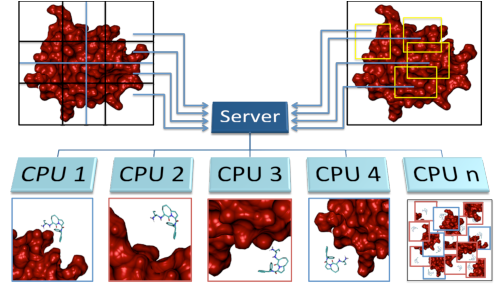
\includegraphics[width=0.65\linewidth]{images/Romain/fig1-color}
	\caption{Exemple d'un schéma de décomposition parallèle}\label{fig:romain-fig1}
\end{figure}

\subsection{Décomposition Géométrique Arbitraire}
Vu la nature des données utilisées en entrée pour le docking, nous avons initialement étudié une stratégie de décomposition géométrique qui consiste à découper la grille d'affinité 3D en plusieurs boîtes plus petites, chacune couvrant un secteur de la protéine. Cette stratégie considère une décomposition géographique régulière de telle manière que le nombre de tâches (boîtes) ont une taille similaire, permettant ainsi la génération de $n^3$ sous-grilles : 8 (2x2x2), 27 (3x3x3), 64 (4x4x4), etc. Le choix du bon nombre de découpages dépend à la fois du gain  en parallélisme mais aussi de la liberté de mouvement du ligand à l'intérieur d'une grille. 
En effet, on peut espérer un gain de performance du fait de pouvoir déployer en parallèle les différentes sous-grilles comme des tâches de calcul indépendantes. Toutefois, un nombre trop important de découpages aura pour effet la génération de sous-grilles "inutiles" car elles couvrent que des zones inaptes à la recherche de points d'amarrage (espace non connecté à la surface de la protéine, "intérieur" de la protéine, etc.). De plus, une boîte 3D trop petite peut empêcher le positionnement du ligand et donc rendre l'évaluation de l'amarrage impossible.

Un autre inconvénient de cette technique est que le découpage se fait de manière arbitraire, sans prendre en compte les spécificités de la surface de la protéine. Par exemple, les "cavités" présentes dans la surface de la protéine sont souvent des bons sites pour l'amarrage, mais un découpage arbitraire qui l'ignore peut simplement scinder cette cavité en deux et la rendre bien moins intéressante vis-à-vis de l'algorithme de docking. De même, l'évaluation de docking se fait en considérant que le ligand se trouve totalement à l'intérieur de la sous-grille : n'importe quelle conformation où des atomes ligand dépassent la grille serait invalide et donc ignorée. 

\subsection{Décomposition Géométrique avec Superposition}
Les inconvénients de la décomposition géométrique arbitraire cités dans la section précédente nous ont conduit à développer une technique alternative de découpage qui préserve la liberté de placement des ligands et permet une couverture intégrale de la surface de la protéine. Cette technique consiste à effectuer un découpage avec superposition entre les sous-grilles voisines, de manière à pouvoir évaluer le placement du ligand même sur les zones proches des bords des sous-grilles. Bien sûr, cette superposition est dépendante de la taille des ligands, permettant ainsi une configuration qui optimise l'utilisation des ressources pour chaque pair protéine-ligand. 

Ainsi, dans le cadre du travail effectué, nous avons considéré deux valeurs de référence pour la superposition. La superposition entre deux boîtes serait d'un tiers de la longueur de la boîte si la longueur du ligand est inférieure à cela. Dans le cas contraire, la superposition correspond à la longueur du ligand. Grâce à cette configuration, le ligand a une liberté complète de placement (rotation, translation, etc.) et on peut effectuer une recherche exhaustive sur l'espace d'amarrage. Dans l'exemple illustré dans les prochaines sections nous utilisons aussi un schéma de décomposition en douze parties, 3x2x2 (où 3 correspond à l'axe principal de la protéine) et avec une superposition d'1/3 sur chaque sous-grille. 

\subsection{Recherche de Cavités}
Comme indiqué précédemment, l'amarrage des ligands est favorisé par la présence de cavités dans la surface de la protéine \cite{Ghersi2009,Hetenyi2011}, or les méthodes de découpage par décomposition ne prennent pas ces facteurs en compte. En effet, même avec la décomposition avec superposition, l'algorithme génétique utilisé pour la recherche de points d'amarrage ne fait que parcourir la surface sans un objectif précis. 

Nous pouvons améliorer la précision de notre docking inversé en effectuant la détection des zones avec cavités, par exemple à l'aide d'un programme dédié à ce fin, l'application Fpocket \cite{Guilloux09a}. La prise en compte des zones avec un plus grand potentiel peut augmenter la performance du docking inversé car cela nous permet de concentrer la recherche sur une zone plus spécifique. L'inconvénient est que son application nécessite un réglage fin des paramètres afin d'inclure les spécificités des protéines et de ne pas exclure des zones avec un potentiel moindre mais réel. 

Ainsi, au lieu de se reposer uniquement sur la recherche de cavités, notre travail a misé sur la complémentarité entre celle-ci et la décomposition géométrique avec superposition. En plus de générer des tâches de calcul pour les différentes sous-grilles issues de la décomposition géométrique, nous générons aussi des recherches ciblées sur les cavités identifiées par FPocket. Ces paramètres permettent une meilleure couverture des zones avec un plus grand potentiel (car couvertes par les deux techniques), tout en limitant le nombre de tâches de calcul supplémentaires.


\section{Gestion et Déploiement des Tâches de Calcul}

Les techniques de découpage présentées dans la section précédente permettent la parallélisation du traitement d'un couple protéine-ligand. Dans le cas du docking inversé, ce parallélisme dit "interne" doit être associé à la génération et au traitement des multiples tâches de calcul issues de chaque combinaison entre un ligand cible et la base de données de protéines recherchée. Enfin, les tâches de préparation des données (génération des sous-grilles, définition des paramètres, regroupement des résultats, etc.) doivent aussi être prises en compte. 

Il faut noter que la présence de tâches de différentes natures (préparation des grilles, criblage virtuel, détection de cavités) rendent la gestion des tâches un peu moins évident. Même les tâches de nature similaire peuvent présenter des variations selon la nature des données à traiter. Si nous prenons par exemple les tâches de criblage virtuel, le temps d'exécution dépend du degré de liberté des peptides à l'intérieur des boîtes 3D : une boîte découpée "à l'intérieur" de la protéine n'aura aucune surface exploitable et sera rapidement écartée.    

Pour toutes ces raisons, nous avons créé deux implémentations visant la gestion et le déploiement des tâches, toutes les deux intégrées à l'outil AMIDE \cite{Vasseur2015}. Dans le premier cas, une plateforme générique qui gère tout seule l'ensemble des tâches a été conçue. Dans le deuxième cas, une partie des responsabilités est déléguée aux gestionnaires de tâches des \textit{clusters}, simplifiant ainsi son exécution dans les environnements déjà pourvus de tels outils.

\subsection{Plateforme Générique}

Vu les besoins de parallélisme interne et externe, nous avons dans un premier moment spécifié et développé une plateforme générique basée sur le langage Python et capable d'exploiter le parallélisme multi-c{\oe}ur et multi-machine pour le docking inversé. 

Ainsi, un ensemble de scripts Python a été créé afin d'automatiser toutes les étapes liées à la préparation et à l'exécution du docking inversé. Parmi ces étapes nous pouvons citer :
\begin{itemize}
	\item[\textbf{(i)}] l'acquisition des fichiers PDB qui décrivent les protéines et ligands, 
	\item[\textbf{(ii)}] la préparation des fichiers PDB afin de sélectionner les structures cible, 
	\item[\textbf{(iii)}] l'extraction des coordonnées pour la création des grilles d'affinité, 
	\item[\textbf{(iv)}] la décomposition des grilles et 
	\item[\textbf{(v)}] le déploiement des tâches de calcul. 
\end{itemize}

Les étapes (i) et (ii) concernent majoritairement la manipulation de fichiers et le \textit{parsing} des informations, alors que les étapes  (iii) et (iv) sont liées à l'exécution de Autogrid, un outil qui fait partie de la suite Autodock et qui permet la création des grilles pour le docking. Selon la stratégie de décomposition retenue, l'étape (iv) peut créer une ou plusieurs grilles correspondant au découpage 3D. Dans le cas où l'on rajoute l'approche par recherche de cavités, il faut rajouter des grilles 3D générées  autour des zones identifiées par le logiciel Fpocket. 


\begin{figure}
	\centering
		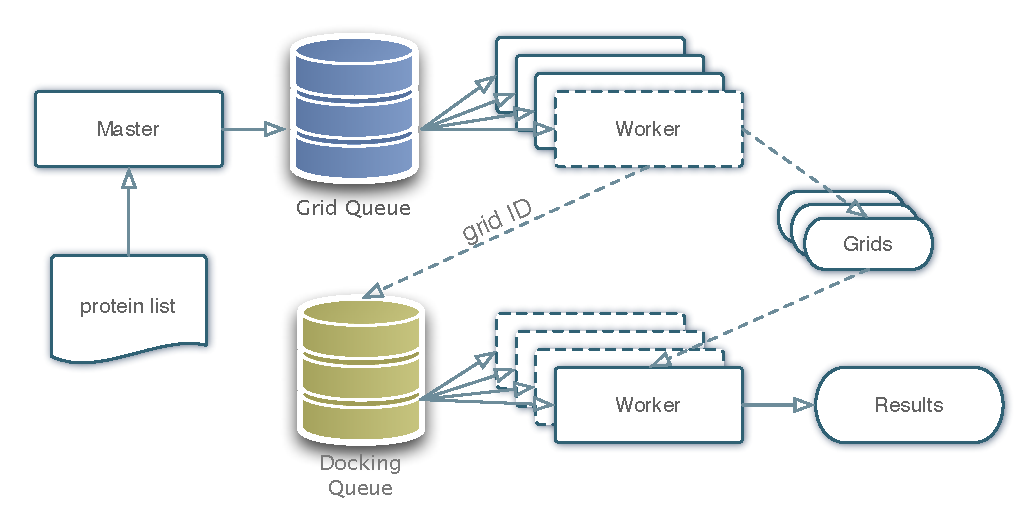
\includegraphics[width=0.5\linewidth]{images/Romain/fig3-color}
	\caption{Représentation du flot d'exécution dans l'architecture distribuée}\label{fig:romain-fig3}
\end{figure}


Pour cela, la plateforme utilise une architecture distribuée maître-esclave avec gestion d'une file d'exécution contenant les identifiants des tâches (task ID) et accessible en mode "sac de tâches" (\textit{bag of tasks} en anglais). Grâce à cette stratégie, les différents esclaves obtiennent une ou plusieurs tâches à exécuter, selon le nombre de c{\oe}urs de calcul disponibles. Pour être plus exacte, dans cette architecture nous trouvons deux files d'exécution, l'une dédiée à la préparation des sous-grilles et l'autre dédiée à l'exécution des tâches de docking. La première file est alimentée par le maître qui, à partir des paramètres d'entrée, indique aux esclaves les différentes protéines à analyser et aussi les stratégies de découpage à mettre en place, ainsi que la génération des sous-grilles avec l'outil Autogrill de la suite Autodock. Les esclaves doivent d'abord finir toutes les tâches dans cette file avant de passer à la file suivante.

Pour plus d'efficacité, la deuxième file d'exécution n'est plus alimentée par le maître mais directement par les esclaves. Lorsque ceux-ci finissent la préparation d'une tâche de la première file, il suffit de déposer le TaskID correspondant dans la deuxième file d'exécution. La Figure \ref{fig:romain-fig3} illustre le flot d'exécution de ces deux étapes.  


\subsection{Optimisation aux Clusters HPC}

 L'architecture distribuée présentée ci-dessous est adaptée à une exécution sur tout type de réseau d'ordinateurs (\textit{cluster}, infrastructures \textit{cloud}, \textit{grid} pervasif, etc.). Toutefois, il est possible d'optimiser son fonctionnement sur les \textit{clusters} HPC si on prend en compte l'existence d'un gestionnaire de tâches propre à ces systèmes. En effet, la plupart des \textit{clusters} HPC fait l'usage d'un gestionnaire de tâches afin de garantir la réservation et l'équité d'usage des ressources. Des systèmes tels que PBS \cite{Henderson95}, OAR \cite{Capit2005} ou Slurm \cite{Yoo2003} sont capables de gérer plusieurs files d'exécution ainsi que de déployer des tâches en mode \textit{best effort} de manière à occuper les ressources de calcul lorsque les réservations ne suffisent pas. 
 
 Dans le cas de l'optimisation pour les \textit{clusters} HPC notre stratégie a été d'éliminer la dépendance vis-à-vis d'un n{\oe}ud maître et permettre ainsi l'exécution des tâches indépendantes selon les disponibilités du gestionnaire de tâches. En effet, la présence d'un n{\oe}ud maître était nécessaire afin de gérer les files d'exécution mais aussi de vérifier la terminaison des tâches (garantissant la tolérance aux fautes). Cela oblige donc que le processus maître reste actif pendant toute l'exécution, ce qui impose des problèmes lors de la réservation des ressources destinées au maître (combien de temps faut-il le garder actif ?). Cette limitation est encore plus importante dans le cas d'un déploiement \textit{best-effort}, où la terminaison des tâches risque d'être fortement étalée au gré de l'occupation des ressources. Comme les gestionnaires de tâches des \textit{clusters} HPC sont capables de détecter une tâche interrompue et la relancer, il suffit de soumettre dans une même tâche les paramètres nécessaires à la génération des sous-grilles et à leur docking. 
 
 Grâce à cette optimisation, l'outil AMIDE issu de ces travaux est capable d'effectuer le docking inversé autant dans un \textit{cluster} que dans un agglomérat de machines indépendantes.
 
 \section{Évaluation Pratique}
 
 Lors de la mise en place de l'outil AMIDE nous avons exécuté plusieurs expériences dans le but de valider notre approche de travail. L'un de ces tests consistait à évaluer la précision des stratégies de décomposition en étudiant un complexe ligand(X23)-protéine(3CM2) bien connu dans la littérature. La comparaison s'est fait par rapport à la technique classique du \textit{blind docking} mais aussi par rapport à des données expérimentales obtenues par cristallographie. Dans un deuxième moment, nous avons conduit des tests de performance dans lesquels le docking inverse était déployé sur un large ensemble de protéines issues de la bibliothèque PDB.
 
Toutes les expériences ont été conduites sur le \textit{cluster} Clovis du centre de calcul ROMEO à Reims. Clovis était un \textit{cluster} hybride avec 36 n{\oe}uds Westmere-EP (12 c{\oe}urs), 2 n{\oe}uds Nehalem-EX (32 c{\oe}urs), un n{\oe}ud Westmere-EP (12 c{\oe}urs + 2 Fermi C2050 GPUs) et un n{\oe}ud Nehalem-EP (8 c{\oe}urs + GPU Fermi M2090), et au moins 2GB de mémoire par c{\oe}ur. Pour une question de régularité, les expériences ici présentées ont été lancées exclusivement sur les n{\oe}uds Westmere-EP. De plus, afin de mieux évaluer la communication \textit{intra-cluster}, seulement 4 c{\oe}urs de calcul ont été utilisés par n{\oe}ud.
 
 Ainsi, pour la première expérience, nous avons initialement exécuté un blind docking de la protéine 3CM2 et du ligand X23. Comme illustré en  Figure \ref{fig:blind}, le blind docking a permis la détection de la cavité et d'une conformation presque identique à celle obtenue par cristallographie (différence RMSD de 1.60 Angstroms seulement).
 
 \begin{figure}[h]
 	\centering
 		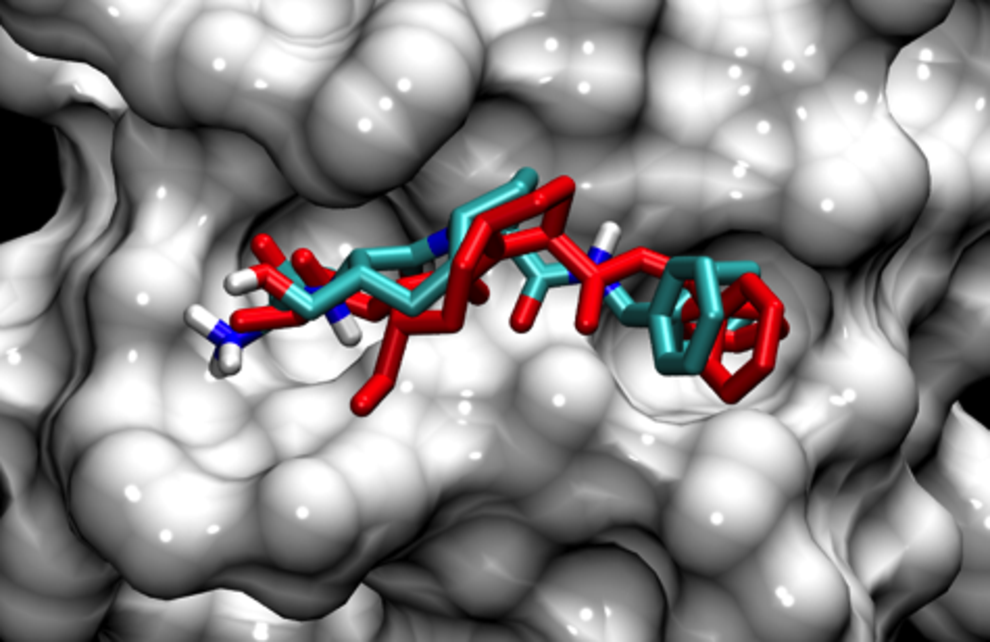
\includegraphics[width=0.75\linewidth]{images/Romain/fig4-color} 
 		\caption{Placement du ligand selon la méthode cristallographique (rouge) et par blind docking (vert)}\label{fig:blind} %\vspace{-0.3cm}
 \end{figure}
 
 \begin{table}
 	\begin{center}
 		\caption{Tableau comparatif des précisions du docking de 3CM2 selon les stratégies de décomposition et le nombre d'itérations. La distance RMSD est comparée à la pose cristallographique et les énergies de liaison à celles obtenues par la méthode blind docking.}\label{tab:rmsd}
 		\begin{tabular}{|c|c|c|c|}
 			\hline 
 			$\Delta G$ blind docking & Nombre d'itérations & énergie de liaison $\Delta G$ & RMSD  \\ 
 			($kcal.mol^{-1}$)  &  & ($kcal.mol^{-1}$) &  (\AA{}) \\
 			\hline 
 			\multirow{3}{*}{$\Delta G = -10.27$}  & 20 & $\Delta G_{12} = -10.09$ & 1.79 \\ \cline{2-4}
 			& 50 & $\Delta G_{pocket} = -10.11$ & 1.86 \\ \cline{2-4}
 			& 70 & $\Delta G_{pocket} = -10.39$ & 1.62 \\ \cline{2-4}
 			\hline 
 		\end{tabular} 
 	\end{center}
 	%\vspace{-0.3cm}
 \end{table}
 
Le découpage avec le meilleur score d'énergie de liaison est celui en $n = 12$, comme illustré en Figure \ref{fig:cuts}. Avec seulement 20 itérations, ce type de décomposition a permis l'obtention d'un placement similaire à celui de la méthode blind docking (voir Table \ref{tab:rmsd}). Les autres formats de découpage ont réussi à placer le ligand dans la cavité cible, mais leurs résultats en termes d'énergie de liaison et de distance RMSD ne sont pas suffisants. La méthode de recherche de cavités a aussi permis le placement du ligand avec une bonne précision, au bout de 50 itérations. 


 
 \begin{figure}[h]
 	\centering
 		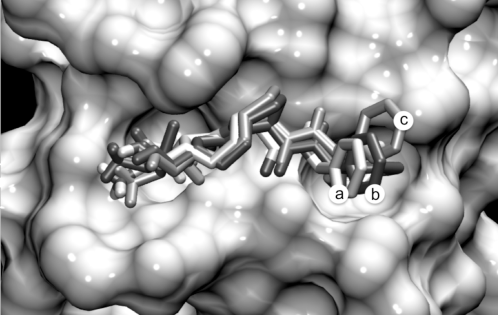
\includegraphics[width=0.75\linewidth]{images/Romain/fig5-bw} 
 		\caption{Comparaison entre la pose blind docking (a) et celle d'un découpage à $n=12$ (b) et par recherche de cavités (c). }\label{fig:cuts} %\vspace{-0.3cm}
 \end{figure}

\begin{figure}
	\centering
		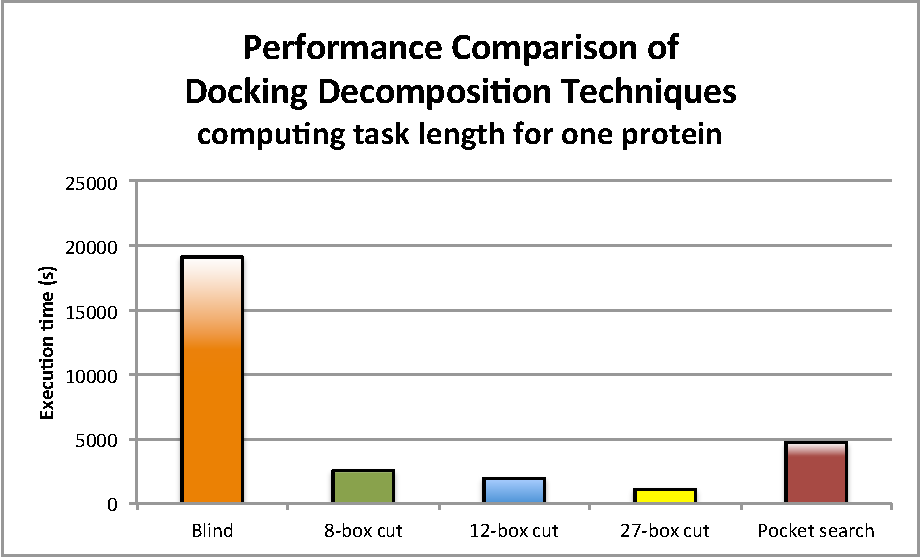
\includegraphics[width=0.5\linewidth]{images/Romain/fig7-color}
		\caption{Comparaison des temps d'exécution pour les tâches issues des différentes méthodes de découpage}\label{fig:performance} %\vspace{-0.3cm}

\end{figure}

%\begin{figure}[h]
%	\begin{center}
%		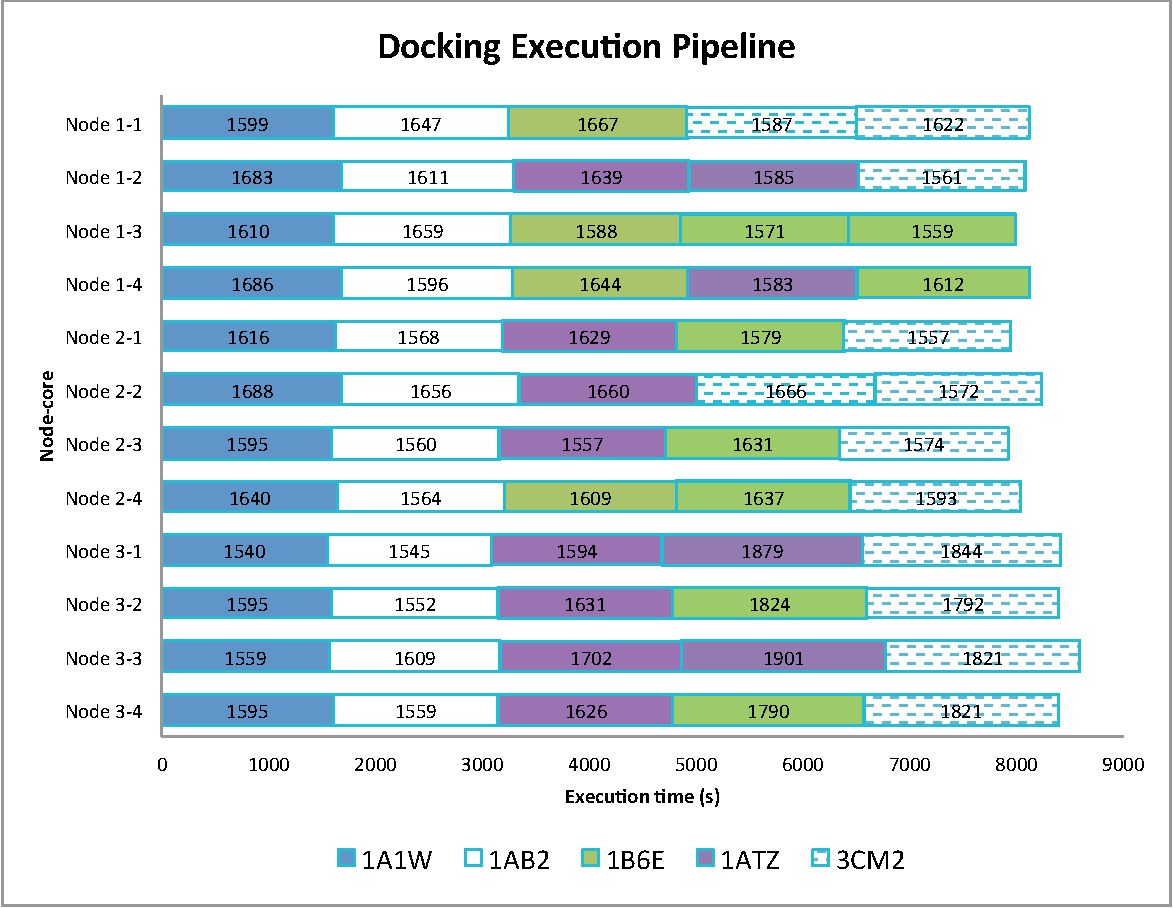
\includegraphics[width=0.5\linewidth]{images/Romain/fig8-color} 
%		\caption{Distribution de la charge lors du docking de 5 protéines (la durée de chaque exécution est indiquée dans les blocks)}\label{fig:balance}\vspace{-0.5cm}
%	\end{center}
%\end{figure} 

 
Dans un deuxième moment nous avons effectué le docking inversé du ligand X23 sur un ensemble de 100 protéines issues de la base PDB. Ici, l'utilisation du découpage a permis une  meilleure utilisation des ressources grâce à l'équilibrage de charge %(voir Figure \ref{fig:balance}) 
mais aussi meilleure prise en charge de la tolérance aux fautes. En effet, la Figure \ref{fig:performance} affiche la durée moyenne d'exécution d'une tâche selon les différentes méthodes considérées dans ce travail. Ainsi, une exécution de type blind docking nécessitait plus de 5h30, et toute interruption oblige la réexécution complète de la tâche. À l'opposé, l'interruption d'une tâche issue d'une décomposition en 12 parties ne demande qu'une demi-heure de ré-exécution, en cas de défaillance.  


 

\section{Bilan et Perspectives} \label{sec:disc}

Les travaux présentés dans ce chapitre démontrent l'intérêt des mécanismes de gestion de l'exécution distribuée lorsque les tâches de calcul sont hétérogènes. En effet, c'est l'un des types de hétérogénéité les plus simples à gérer et dont le besoin se fait sentir de plus en plus à cause de la multiplication de ressources parallèles à notre disposition (c{\oe}urs de calcul, GPUs, etc.). 

L'expérience avec le développement de la plateforme AMIDE a aussi exposé une facette moins connue de la parallélisation des applications : l'étude des stratégies pour la parallélisation lorsqu'on ne peut pas modifier le code source de l'application. En effet, la communauté HPC a souvent tendance à négliger ce type de contrainte alors qu'on est de plus en plus confrontés à des situations où la réécriture de l'application métier est trop complexe.  

D'un point de vue performance et volume de calcul, plusieurs autres campagnes de simulation ont été conduites ces dernières années, portant sur d'autres peptides d'intérêt pharmaceutique tels que les ligand BAT et NGH, inhibiteurs du MMP-3, une protéine associée à certaines maladies telles que l'arthrite et la métastase des tumeurs. L'intégration avec le gestionnaire de tâches Slurm du Centre de Calcul ROMEO rend plus simple le déploiement de ces campagnes.

Bien évidemment, ça a été aussi une expérience humaine très enrichissante, du fait de pouvoir travailler avec des chercheurs et un doctorant issus d'autres domaines que l'Informatique. Ceci a affecté non seulement les méthodes et outils de travail (par exemple, le choix des langages de programmation) comme a permis la confrontation de différentes perceptions des mécanismes de publication et de divulgation scientifique. Cette proximité avec des chercheurs d'autres domaines est une spécificité de la recherche HPC à Reims, où des chercheurs en chimie, biologie ou physique côtoient les informaticiens au sein des plateaux techniques de la Maison de Simulation de Champagne-Ardenne (Centre de Calcul ROMEO, Centre Image et P3M - Plateau de Modélisation Moléculaire Multi-échelles). Cette expérience m'a encouragé à poursuivre l'ouverture à d'autres domaines, comme, par exemple, le projet CAPES-Cofecub MESO mené en partenariat avec des chercheurs en physique de l'atmosphère.

Parmi les perspectives, on peut citer la poursuite de la collaboration autour de AMIDE qui prend la forme d'un proposition de projet ANR en 2017. Ce projet porte sur la possibilité d'intégrer les N-glycosylation aux simulations effectuées sur les protéines de la matrice extra cellulaire. Les N-glycosylation sont des importants marqueurs dans les études sur le diabète et les récepteurs de l'insuline et, pour certaines protéines, les sites sont nombreux et les données expérimentales ne permettent pas toujours de connaître le nombre et les types de N-glycosylation portés par la molécule. Ma participation à ce projet relève de l'adaptation et de l'évolution de la plateforme AMIDE afin de déployer ces simulations à plus grande échelle.  


 







